\documentclass{article}

\author{Tran Van Tan Khoi}

\title{Homework Report Week \#1}

\usepackage[T1]{fontenc}
\usepackage[utf8]{inputenc}
\usepackage[a4paper,top=2cm,bottom=2cm,left=3cm,right=3cm,marginparwidth=1.75cm]{geometry}
\usepackage[colorlinks=true, allcolors=blue]{hyperref}
\usepackage{bookmark}
\usepackage{graphicx}


\usepackage{tcolorbox}
\tcbuselibrary{theorems}

\newtcbtheorem[number within=section]{theorem}{}%
{colback=green!5,colframe=green!35!black,fonttitle=\bfseries}{th}

\newtcbtheorem[number within=section]{statement}{}%
{colback=blue!5,colframe=blue!35!black,fonttitle=\bfseries}{th}

\newtcbtheorem[number within=section]{example}{}%
{colback=magenta!5,colframe=magenta!35!black,fonttitle=\bfseries}{th}


\begin{document}
    \maketitle

    \section{Introduction}
    
    This week's set of problems focus on writing recursion functions for finding and counting solutions for various classic problems, such as finding the N-th Fibonacci number and solving the N-Queens Problem. The report goes in detail of how I approach such problems. None of the solutions presented here are revolutionary, but rather an reiteration of the most common and typical way one might go on using to solve the problems.


    This report, along with C++ solutions, can be found over at \href{https://github.com/xtrkoi/throwaway-rep}{this Github repo}.

    \begin{figure}[!h]
        \centering
        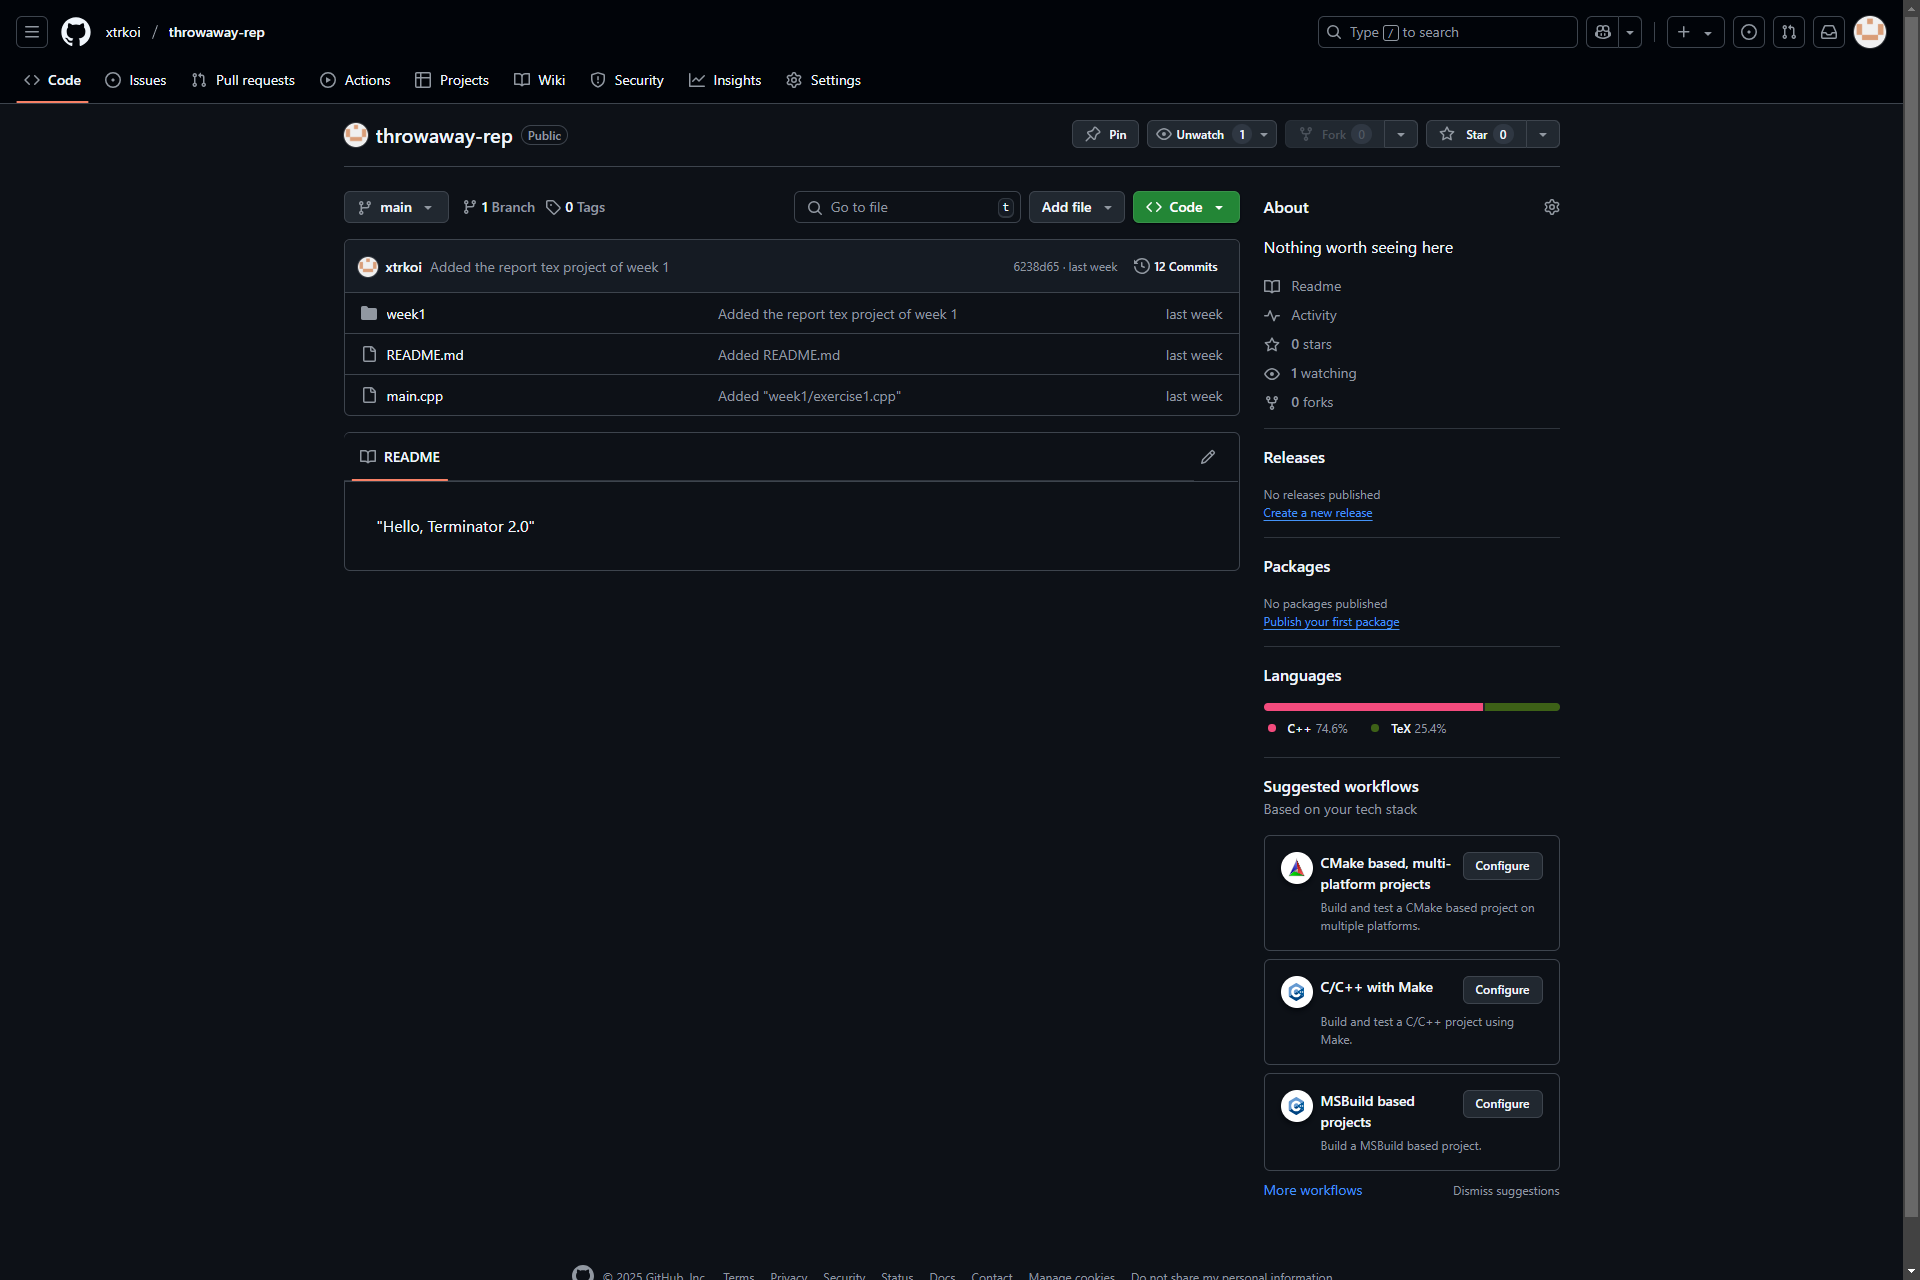
\includegraphics[width=12cm]{figure1.png}\hfil
        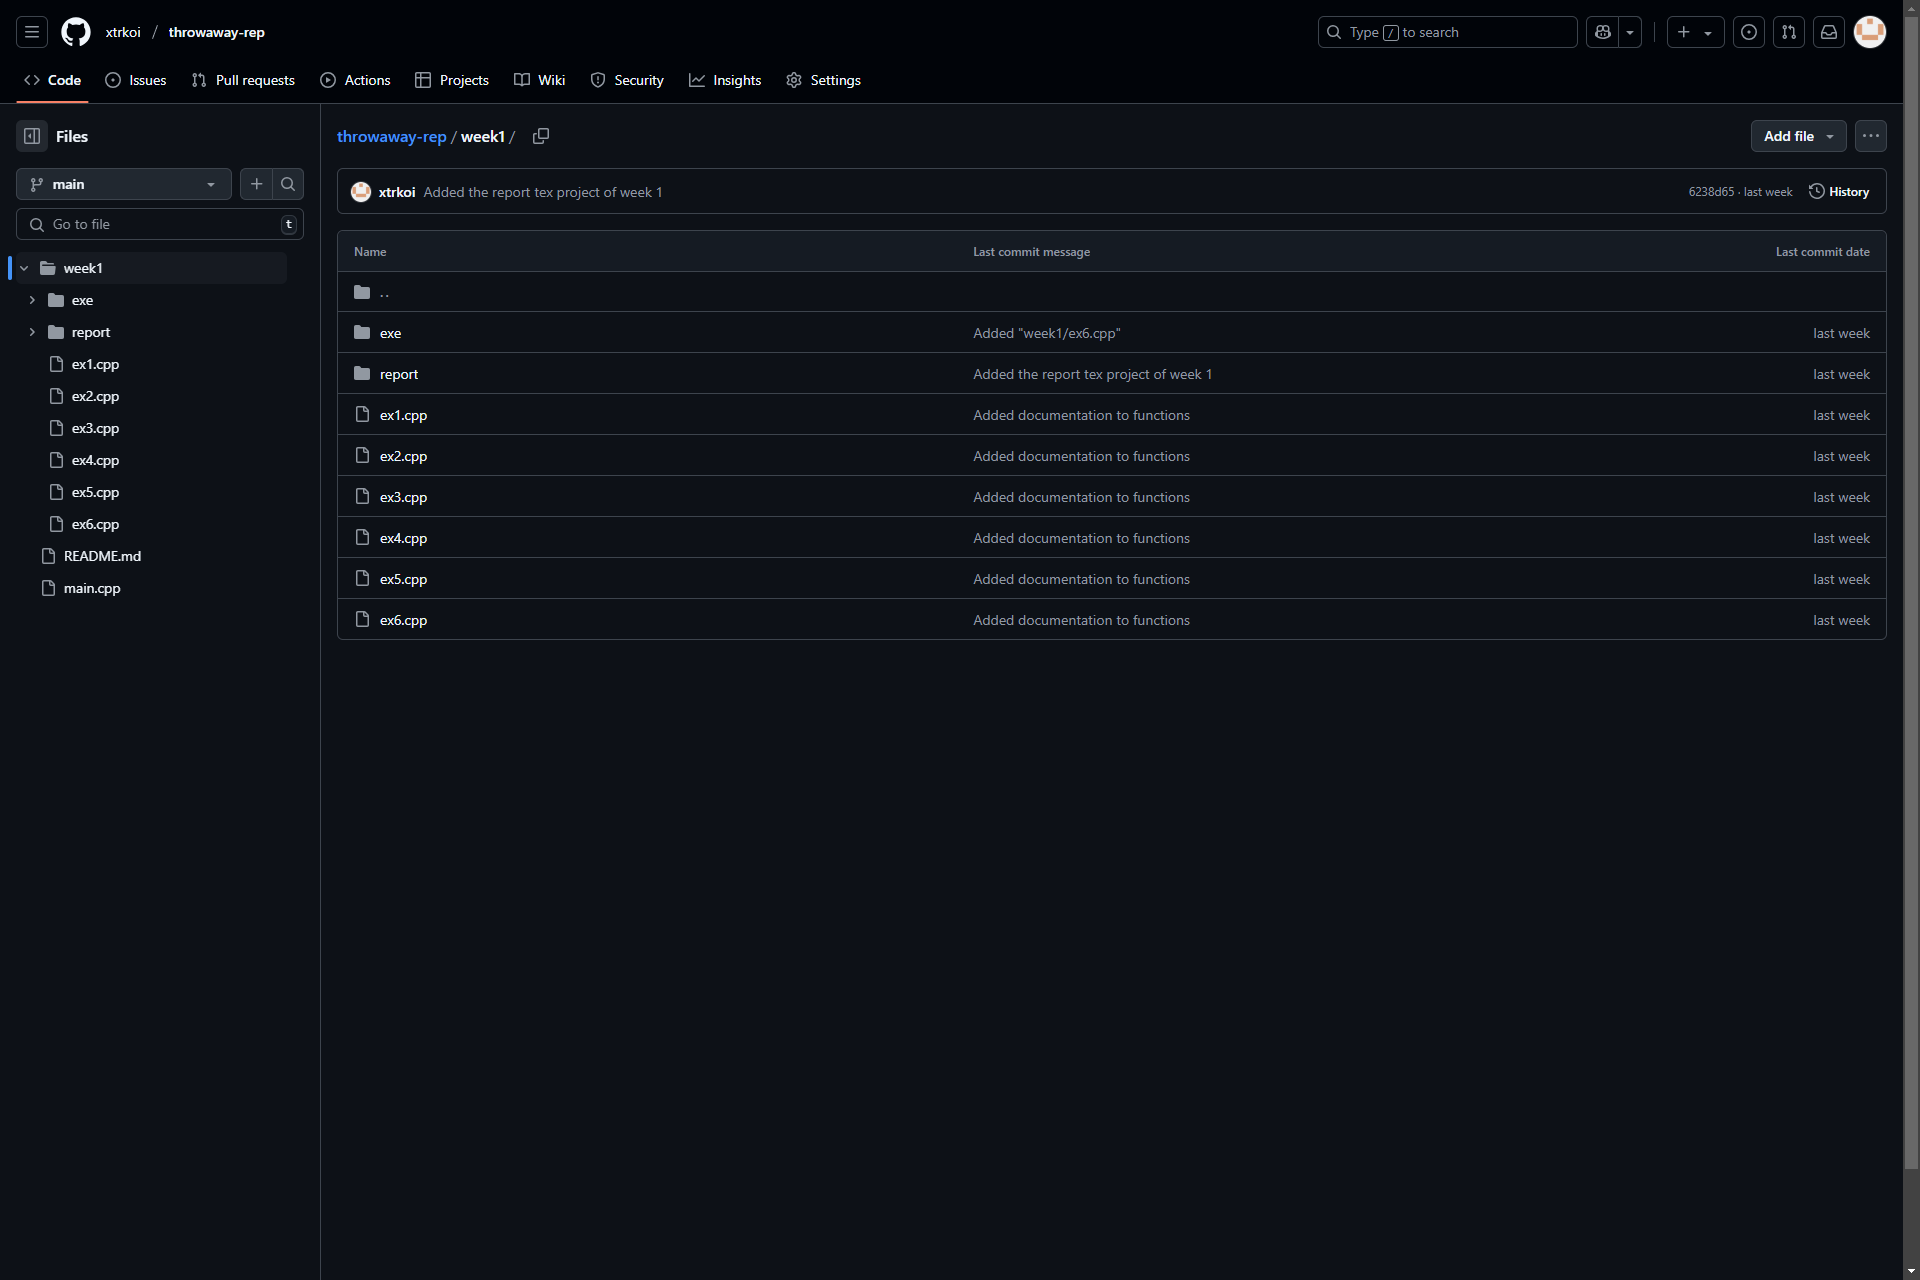
\includegraphics[width=12cm]{figure2.png}
        \caption{Online Github Repository}
    \end{figure}

    \section{The Problems}



    \subsection{Fibonacci Sequence}

    \begin{statement*}{Fibonacci Sequence}{}
        The Fibonacci Sequence is a sequence defined by the recursive formula:

        \begin{equation*}
            \begin{cases}
                F(n) = F(n - 2) + F(n - 1), \quad \forall n \ge 2 \\
                F(0) = 0, F(1) = 1
            \end{cases}
        \end{equation*}

        Given a positive integer $n$, find $F(n)$ using recursion.

        \emph{Input}: A positive $n$ $(n \le 10^6)$.

        \emph{Output}: A list of numbers $\{F(i) | i \in [0, n)\}$.
    \end{statement*}

    \emph{Approach.} As a formula is already given, a direct approach would be implementing it with a programming language that support recursion, with \emph{C++} being one of them. However, to print a list of the sequence, we need to keep track of the next number in the sequence to print. Here we leverage $memoization$, a technique in which we store intermediate results, saving time and making it more convenient to output. In this case, simply saving $F(n)$ to an array $f[n]$ will do the trick.

    \subsection{N-th Factorial}

    \begin{statement*}{N-th Factorial}{}
        Given the factorial of $n$: $n! = \prod_{x=1}^{n} x = 1 \cdot 2 \cdot \cdots \cdot (n - 1) \cdot n$, and a positive integer $n$, find $n!$ using recursion.
        
        \emph{Input}: A positive $n$ $(n \le 20)$.

        \emph{Output}: $n!$.
    \end{statement*}

    \emph{Approach.} Define $F(n)$ as the factorial of $n$, with $F(0) = 1$, we obtain $F(n) = F(n - 1) \cdot n$. And the rest is implementation, with a reminder that $20! \approx 2.43 \cdot 10^{18}$ can exceed the maximum value that \emph{int} can hold, so use \emph{long long} instead.

    \subsection{Generating Binary Strings}

    \begin{statement*}{Generating Binary Strings}{}
        Define a \emph{binary string} as a sequence of digits, each being either $0$ or $1$. Given a positive integer $n$, for each $i$ in $[0, 2^n - 1]$, print a binary string which is the binary representation of $i$.

        \emph{Input}: A positive integer $n$ $(n \le 20)$.

        \emph{Output}: $2^n$ seperate lines, each line $i$ contains the binary representation of $i$.
        
    \end{statement*}

    \begin{example*}{Example}{}
        \emph{Input}:

        \begin{verbatim}
            3
        \end{verbatim}

        \emph{Output}:

        \begin{verbatim}
            000
            001
            010
            011
            100
            101
            110
            111
        \end{verbatim}
    \end{example*}

    \emph{Approach.} This is a fundamental application of $backtracking$. Define $B(x)$ as a binary string of length $x$. When $x < n$, there are only two options, adding $0$ or $1$ to the end of the string $B(x)$ to create $B(x + 1)$. When $x = n$, simply print the string then return the function.

    \subsection{Tower of Hanoi}

    \begin{statement*}{Tower of Hanoi}{}
        Three towers reside next to each other. $n$ disks in order of decreasing radius are placed on the leftmost tower, the other two are empty. Each move consists of picking up the top most disk of a tower and move it onto another tower that is either empty or the top most of that tower has bigger radius. Find a list of moves to transport all disks from the left tower to the right tower.
    \end{statement*}

    \emph{Approach.} Backtracking. We name the towers $A, B,$ and $C$, with the disks starting on tower $A$. Isolate the problem by only considering two disks on tower $A$. To move both of them to tower $C$, move the smaller disk to tower $B$, the larger disk to tower $C$, then the smaller disk to tower $C$. All of this can be implemented by a recursive function.

    \subsection{Sorted Array Check}

    \begin{statement*}{Sorted Array Check}{}
        Given an array of $n$ integers $(n > 0)$, check if the array is sorted in ascending order.
    \end{statement*}

    \emph{Approach.} Define the function $f(i)$ to returns \emph{true} if the array is sorted from index $1$ to index $i$. Then $f(n)$ is $true$ if and only if $f(n - 1)$ is true and $a_{n - 1} \le a_n$.

    \subsection{N-Queens Problem}

    \begin{statement*}{N-Queens Problem}{}
        Count the number of ways $n$ queens can be placed on a $n \times n$ chessboard without any two queens attacking each other. Two queens are considered attacking if both of them are on the same row, column or diagonal.
    \end{statement*}

    \begin{example*}{Example}{}
        \emph{Input}:

        \begin{verbatim}
            8
        \end{verbatim}

        \emph{Output}:

        \begin{verbatim}
            92
        \end{verbatim}
    \end{example*}

    \emph{Approach.} Backtracking. Place the queens row by row. This way, each newly placed queen don't attack any queens placed before on the same row. To check for attacking columns and diagonals, use three arrays.

    \section{Conclusion}

    This handful collection of problems help improving the logical processing of certain problems where recursion can be applied and implementing recursion using \emph{C++} programming language. The problems range from elementary to slightly mind-bending but nothing too extreme. By having a deep understanding of how the problems arise in other applications, one can find how recursion play many roles in programming paradigms.

\end{document}